\documentclass[10pt]{article}
\usepackage{graphicx}
\DeclareGraphicsExtensions{.pdf,.png}
\graphicspath{{./figures/}}
\usepackage{url}
\usepackage{epsfig} 
\usepackage{amssymb}
\usepackage{amsmath}
\usepackage{amsfonts}
\usepackage{floatflt}
\usepackage{caption}
\usepackage{subcaption}
\setcounter{secnumdepth}{5}
\setcounter{tocdepth}{5}


\setlength{\oddsidemargin}{0in}   % 10pt is 1.875 for margins in latex
\setlength{\evensidemargin}{0in}
\setlength{\textwidth}{7in}
\setlength{\textheight}{9in}
\setlength{\topmargin}{-0.5in}

\newcommand{\ignore}[1]{}

\thispagestyle{empty}
\begin{document}
\date{}

\title{Governance of Web APIs in Modern Cloud Computing Environments}

\author{Hiranya Jayathilaka\\
Department of Computer Science\\
Univ. of California, Santa Barbara, CA\\
Email: hiranya@cs.ucsb.edu
}
\maketitle

\section{Introduction}
\textbf{Cloud computing turns compute infrastructures, programming platforms and software systems
into online utility services that can be easily shared among many users~\cite{hassan2011demystifying,Mell:2011:SND:2206223}.}
It enables processing and storing data on large, managed infrastructures and 
programming platforms, that can be accessed remotely via the internet. This provides an
alternative to running applications on local servers, personal computers, and mobile devices,
all of which have strict resource constraints. 
Today, cloud computing technologies can be obtained from a large and growing number of providers.
Some of these providers offer hosted cloud platforms that can be used
via the web to deploy applications without installing any physical hardware 
(e.g. Amazon AWS~\cite{amazon-aws-web}, Google App Engine~\cite{gae}, Microsoft Azure~\cite{azure-web}). Others
provide cloud technologies as downloadable software, which users can install
on their computers or data centers to set up their own private clouds 
(e.g. Eucalyptus~\cite{eucalyptus09}, AppScale~\cite{6488671}, OpenShift~\cite{openshift}).

\textbf{Cloud computing model provides high scalability, high availability and enhanced levels of 
user productivity.} Cloud platforms run on large resource pools, typically in one or more
data centers managed by the platform provider. Therefore cloud platforms have access to a vast
amount of hardware and software resources. This enables cloud-hosted applications
to scale to varying load conditions, and maintain high availability. Moreover, by offering resources
as utility services, cloud computing is able to facilitate a cost-effective, on-demand
resource provisioning model that greatly enhances user productivity. 

\textbf{Over the last decade cloud computing technologies have enjoyed explosive growth, 
and near universal adoption due to their many benefits and 
promises~\cite{Antonopoulos:2010:CCP:1855007,Pinheiro:2014:ACC:2618168.2618188}.} 
Industry analysts project that the cloud computing market value will exceed \$150 billion
by the year 2020~\cite{cloud-growth}.
A large number of organizations
run their entire business as a cloud-based operation (e.g. Netflix, Snapchat). For startups
and academic researchers who do not have a large IT budget or a staff, the cost-effective 
on-demand resource provisioning model of the cloud has proved to be indispensable.
The growing number of academic conferences and journals dedicated to discussing
cloud computing is further evidence that cloud is an essential branch in the field
of computer science.

\textbf{Despite its many benefits, cloud computing has also given rise to several application
development and maintenance challenges that have gone unaddressed for many years.}
As the number of applications deployed in cloud platforms continue to increase these
shortcoming are rapidly becoming conspicuous. We highlight three such issues.
 
\textbf{Firstly, cloud platforms lack the ability to enforce developer best practices
and administrative conformance on deployed user applications.} The developer best practices 
are the result of decades of software engineering research, and
include code reuse, proper versioning of software artifacts, dependency management
between application components, and backward compatible software updates. Administrative
conformance refers to complying with various development and maintenance standards
that an organization may wish to impose on all of their production software.
Cloud platforms do not provide any facilities that enforce such developer practices or
administrative standards. Instead, cloud platforms
make it extremely trivial and quick to deploy new applications or update existing
applications (i.e. roll out new versions). The resulting speed-up of the development cycles combined with the lack of 
oversight and verification, makes it extremely difficult for 
IT personnel to manage large volumes of cloud-hosted applications.

\textbf{Secondly, today's cloud platforms do not provide support for establishing 
service level objectives (SLOs) regarding the performance of deployed applications.} 
A performance SLO specifies a bound on application's response time (latency). 
Such bounds are vital for developers 
who implement downstream systems that consume the cloud-hosted applications,
and cloud administrators who wish to maintain a consistent quality of service
level. However, when an application is implemented for
a cloud platform, one must subject it to extensive performance testing in order
to comprehend its performance bounds; a process that is both 
tedious and time consuming. The difficulty in understanding the performance 
bounds of cloud-hosted applications is primarily due to the very high level of 
abstraction provided by the cloud platforms. These abstractions shield many details 
concerning the application runtime, and without visibility into such low level application 
execution details it is impossible
to build a robust performance model for a cloud-hosted application. Due to this
reason, it is not possible to stipulate SLOs on the performance of cloud-hosted applications. 
Consequently, existing cloud platforms only offer SLOs regarding service availability.

\textbf{Thirdly, cloud platforms do not provide adequate support for monitoring application performance,
and running diagnostics when an application fails to meet its performance SLOs.} 
Most cloud platforms only provide the simplest monitoring and logging features,
and do not provide any mechanisms for detecting performance anomalies or identifying
bottlenecks in the application code or the underlying cloud platform. This limitation has given rise
to a new class of third party service providers that specialize in monitoring cloud applications
(e.g. New Relic~\cite{newrelic}, Dynatrace~\cite{dynatrace}, Datadog~\cite{datadog}). But these 
third party solutions are expensive. They also require code instrumentation, which
if not done correctly, leads to incorrect diagnoses. The perturbation
introduced by the instrumentation also changes and degrades application performance.
Furthermore, the extrinsic monitoring systems have a restricted view 
of the cloud platform, due to the high level of abstraction provided by cloud platform software.
Therefore they cannot observe the complexity of the cloud platform in full, and hence cannot pinpoint
the component that might be responsible for a perceived application performance anomaly.

\textbf{In order to make the cloud computing model more dependable, maintainable and convenient for the users as well
as the cloud service providers, the above limitations need to be addressed satisfactorily.}
Doing so will greatly simplify the tasks of developing cloud applications, and maintaining 
them in the long run. Developers will be able to specify SLOs on the performance of
their cloud-hosted applications, and offer competitive service level agreements (SLAs) to the end users that consume those
applications. Developers as well as cloud administrators will be able to detect performance anomalies
promptly, and take corrective actions before the issues escalate to major
outages or other crises.

\textbf{Our research focuses on addressing the above issues in cloud environments 
using \textit{governance}.} We define governance as the mechanism 
by which the acceptable operational parameters are specified and maintained in a 
software system~\cite{brown2005framing,gartner-soa-gov}. This involves multiple steps:
\begin{itemize}
\item Specifying the acceptable operational parameters
\item Enforcing the specified parameters
\item Monitoring the system to detect deviations from the acceptable behavior
\end{itemize}

To learn the feasibility and the efficacy of applying governance
techniques in a cloud platform, we propose and explore the following thesis
question:
{\bf Can we efficiently enforce governance for cloud-hosted web applications to achieve 
administrative conformance, developer best practices, and performance SLOs through 
automated analysis and diagnostics?} 

\textbf{For governance to be
useful within the context of cloud computing, it must be both efficient and automated.}
Cloud platforms are comprised of many components that have different life cycles
and maintenance requirements. 
They also serve a very large number of users who deploy applications in
the cloud. Therefore governance systems designed for the cloud should scale to handle a 
large number of applications and related software components,
without introducing a significant runtime overhead on them.
Also they must be fully automated since it is not practical for a human administrator to be
involved in the governance process given the scale of the cloud platforms.

Automated governance for software systems is a well researched area,
especially in connection with classic web services and service-oriented architecture 
(SOA) applications~\cite{gartner-soa-gov,soagov,Schepers:2008:LAS:1363686.1363932,5577268,4730489}. 
\textbf{We adapt the methodologies outlined in the existing SOA governance research corpus, so
they can be applied to cloud computing systems.}
These methodologies enable specifying
acceptable behavior via machine readable policies, which are then automatically enforced by
a policy enforcement agent. Monitoring agents watch the system to detect any deviations from
the acceptable behavior (i.e. policy violations), and alert users or follow predefined corrective
procedures. We can envision similar facilities being implemented in a cloud platform to 
achieve administrative conformance, developer best practices and performance SLOs. The operational
parameters in this case may include coding and deployment conventions for the cloud-hosted
applications, and their expected performance levels.

\textbf{In order to answer the above thesis question by developing efficient, automated governance systems,
we take the following three-step approach.}
\begin{itemize}
\item Design and implement a scalable, low-overhead governance framework for cloud platforms,
complete with a policy specification language and a policy enforcer. The governance framework should be
built into the cloud platforms, and must
keep the runtime overhead of the user applications to a minimum while enforcing
developer best practices and administrative conformance.
\item Design and implement a methodology for formulating performance SLOs (bounds)
for cloud-hosted web applications, without
 subjecting them to extensive performance testing or instrumentation. The formulated
SLOs must be correct, tight and durable in the face of changing conditions of the cloud.
 \item Design and implement a scalable cloud application performance monitoring (APM) framework for detecting
violations of performance SLOs. For each
violation detected, the framework should be able to run diagnostics, and identify the potential
root cause. It should support collecting data from the cloud platform
 without instrumenting user code, and without introducing significant runtime overheads.
\end{itemize}

\textbf{To achieve administrative conformance and developer best practices with minimal overhead,
we perform governance policy enforcement when an application is deployed; a technique that we
term deployment-time policy enforcement.} 
We explore the
trade off between what policies can be enforced, and when they can be enforced with respect
to the life cycle of a cloud-hosted application. We show that not all policies
are enforceable at deployment-time, and therefore some support for run-time policy enforcement
is also required in the cloud. However, we find that
deployment-time policy enforcement is efficient, and a governance framework that
performs most, if not all, enforcement tasks at deployment-time can scale
to thousands of applications and policies.

\textbf{We combine static analysis with platform monitoring to establish performance SLOs for
cloud-hosted applications.} Static analysis
extracts the sequence of critical operations (cloud services) invoked by a given application.
Platform monitoring facilitates constructing a historic performance model for the individual operations.
We then employ a time series analysis method to combine these results, and calculate statistical bounds 
for application response time. The performance bounds calculated in this manner
are associated with a specific correctness probability, and hence can be used
as SLOs. We also devise a statistical framework to evaluate the validity period of 
calculated performance bounds.

\textbf{In order to detect and diagnose performance SLO violations,
we monitor various performance events that occur in the cloud platform,
correlate them, and employ statistical analysis to identify anomalous patterns.} Any given statistical
method is only sensitive to a certain class of anomalies. Therefore, to be able to diagnose a wide range of
performance anomalies, we devise an algorithm that combines linear regression, change point
detection and quantile analysis. Our approach detects performance SLO violations in near real time,
and identifies the root cause of each event as a workload change or a performance bottleneck
in the cloud platform. In case of performance bottlenecks, our approach also correctly identifies
the exact component in the cloud platform, in which the bottleneck manifested.

\textbf{Our contributions push the state of the art in cloud computing significantly towards achieving
administrative conformance, developer best practices and performance SLOs.} Moreover,
our work addresses all the major steps associated with software system governance --
specification, enforcement and monitoring. We show that this approach can significantly improve cloud platforms
in terms of their reliability, developer-friendliness and ease of management. We also demonstrate
that the governance capabilities proposed in our work can be built into existing cloud platforms,
without having to implement them from the scratch.

\section{Research Context: API-driven Development Model in the Cloud}
As scalable information technology evolves to a more cloud-like model,
{\em digital assets} (code, data and software environments) 
are increasingly integrated into applications by developers 
as web-accessible services.
This application development model facilitates code reuse and eases the 
assembly of complex systems thereby greatly improving programmer productivity
over non-service-oriented methodologies~\cite{Dan:2008:SSR:1370916.1370923}. 
By composing an application from existing services that 
encapsulate common yet complicated tasks developers are able  
to work at a higher level of abstraction, employ any programming 
language they choose, leverage the work, testing, and quality
assurance of others, and thus innovate faster.  

\begin{floatingfigure}[rb]{2.8in}
\vspace{-0.1in}
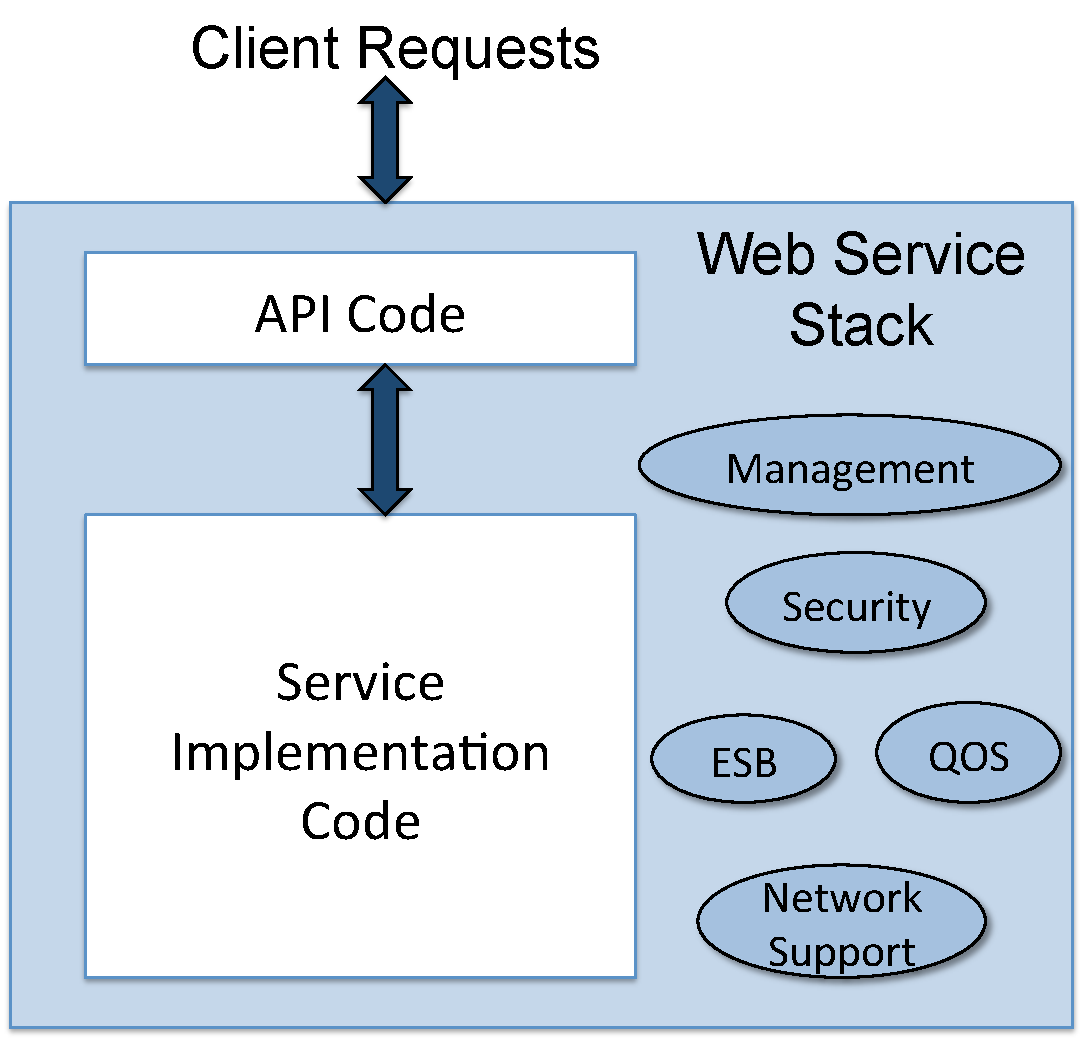
\includegraphics[scale=.34]{stack}
\vspace{-0.08in}
\caption{Web Service Software Components\label{fig:ws-arch}}
\end{floatingfigure}
Production web services consist of three components: API code, service
implementation code, and a web service ``stack'' that implements a container
for combining and deploying the API and service implementation
together ({\em c.f.} Figure~\ref{fig:ws-arch}).
Clients contact the web service container which routes requests to the
API code. The container implements common functions such as 
service management (registration, description, discovery), a service
bus (ESB), and security, among other 
functions.

Increasingly, IT organizations are tasked with deploying and 
maintaining web services as software infrastructure components, hosted in a
shared cloud platform ({\em i.e.} in a way analogous to the manner in which they
would deploy a piece of shared physical infrastructure).  
To achieve economies of scale, these services are shared (in a controlled
way) among the widest possible set of users and client applications.  Indeed,
it is the possibility of Internet-scale sharing that makes this model
attractive from an IT management perspective. As a consequence we 
are witnessing an explosion of web APIs on the Internet today. ProgrammableWeb~\cite{pweb},
the popular online API registry, currently boasts over 12,000 registered APIs and
a near exponential growth rate since 2006.

The modular design of web services inherently separates API, 
service implementation, and container. However, only 
the service implementation and the container is under complete
control of IT. External clients access APIs independently from IT.
Even internally developed client applications may be too numerous and
constantly evolving for IT to track or control given
potentially tens or hundreds of engineering teams and hundreds or 
thousands of APIs.  That is, the decoupling of the API from the 
other components of the web service provides many programmer
benefits, but it also introduces several IT management challenges 
at production scales. 

The confluence of application concerns ({\em e.g.} 
application functionality and productivity) with IT 
concerns ({\em e.g.} life cycle management, security) 
has led to new organizational approaches such as
DevOps~\cite{devops}.  However, 
the technologies that have been developed
to date address the core API
governance challenges incompletely, if at all. 
In particular, new research and technology is needed 
to provide scalable and unified automation to the problem
of implementing and enforcing consistent governance for APIs. 
By using automation to ensure consistency, my goal is to alleviate the 
labor burden associated with uniform policy implementation and SLA enforcement.  

To my knowledge, there is no extant system that automates governance and
SLA enforcement across the life cycle
of an API, across diverse categories of policies, for web
APIs in cloud environments simply and scalably. The goal of my work is to investigate 
new research and to develop
new technologies that do so for the next generation of service ecosystems.

\section{Research Plan}
The type of service ecosystem described in the previous section 
is becoming the norm for modern organizations: cloud-based web APIs, 
complex service relationships, external and
internal service consumers, agile software development, rapid release
cycles, and a host of diverse policies and SLAs that
govern service development, deployment, and use.  
As a result, IT organizations are increasingly responsible 
for deploying, managing, and evolving services
and their APIs as software infrastructure components at scale (10s-100s
of engineering teams, 100s-1000s of APIs/services).  The goal of my work
is to reduce the cost and labor burden of IT management of web services
by automating and simplifying governance (policy specification, 
and enforcement) for a wide range of management functions.

To enable this, I propose to investigate
a holistic solution that leverages, combines, and extends techniques from 
formal methods, programming language analysis, 
language design, runtime systems, and cloud platforms in a new 
and unified way that achieves simplified and uniform specification of,
and end-to-end enforcement of, disparate governance policies and SLAs.
Key components of this research schedule are as follows.

\begin{itemize}
\item {\bf IT management policy enforcement}: I intend to develop a new
model and an architecture that augments existing cloud architectures to
facilitate enforced API governance as a cloud-native feature. This will
facilitate comprehensive enforcement of IT policies both at service
development time and at runtime. This new model will also track the dependencies
between services and ensure that developers adhere to proper naming conventions,
reuse existing APIs as much as possible, and retain backwards-compatibility when
releasing new versions of existing APIs. To that end I will also explore the
requirements for a new policy language that is both easy to use for policy authors
and efficient to process and execute in the cloud (most existing
declarative policy languages are inflexible and hard to program with). The tracked
dependency information will be used to perform impact analysis and point
out potential failures due to API changes, before they occur. Similarly this
model will be able to enforce a wide range of runtime policies involving security,
request rate limiting, caching, load balancing and fail-over routing. In order to fit the
cloud model, the architecture of the policy enforcer needs to be distributed, highly
scalable and highly available.

\item {\bf Simplify the API-based development model}: Developers today need to perform
a large amount of manual work in order to deal with issues pertaining to API discovery,
subscription, evaluation and consumption. But these problems keep getting complicated
as the popularity of cloud computing drives the number of APIs to new heights. In order to
efficiently deal with these issues, and make the API-based development model
simpler, we need new tools and mechanisms that are both powerful and automatic. To
that end I will explore new techniques for automating a wide range of tasks
related to API-based development, with a strong focus on cloud-based development and
deployment environments. This includes research in machine-readable languages for describing
the syntactic and semantic aspects of APIs, tools to auto-generate such specifications by
performing static analysis on service or API code, automated discovery and engagement
protocols for APIs, and formal methods for evaluating APIs for risk, usability and 
developer experience.

\item {\bf Automated QoS and performance analysis}: Service providers today have to perform
a large amount of offline and online testing to understand the performance and QoS characteristics
of their services. I propose using a combination of static analysis and system monitoring as a 
means of obtaining early estimates of service performance levels. Services developed for cloud
platforms rely on core cloud services (e.g. datastore and taskqueue in case of Google App Engine)
and other web services hosted
in the cloud. A through static analysis on the service implementation can reveal these dependencies
and any patterns in invoking them (branches, loops etc.). By combining this information with the
historical performance data of those dependencies, we can make predictions regarding
the performance that can be expected from a web service. We can make these estimates even
more accurate by taking into account the network usage, database growth and other infrastructure
related metrics. Such an approach will enable service developers to better understand what SLAs their
services can support, under which circumstances, and what improvements should be made to their 
service implementations
in order to support more competitive SLAs. This deep insight into the different SLAs
an API can support along with the knowledge on limitations of the target cloud, allow developers
to set up proper redundancy and backup channels, and also to implement graceful degradation
in the event of a catastrophic failure. 

\end{itemize}



\section{Progress and Ongoing Work}
\begin{floatingfigure}[rb]{2.8in}
\vspace{-0.1in}
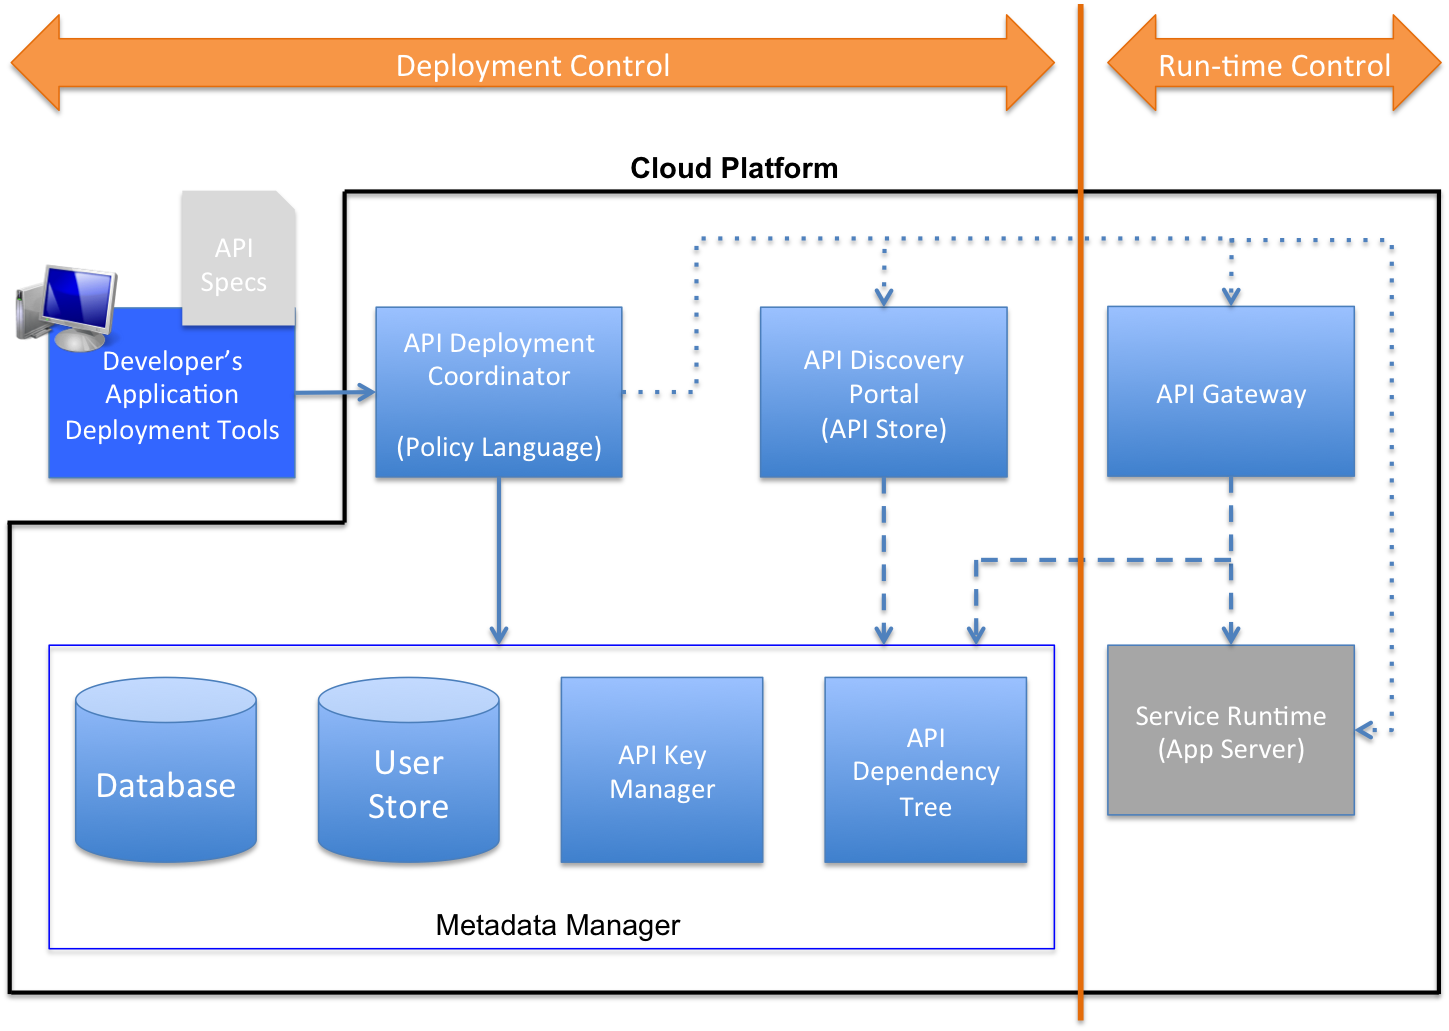
\includegraphics[scale=.27]{eager_design_2}
\vspace{-0.08in}
\caption{EAGER architecture\label{fig:eager}}
\end{floatingfigure}

I started this research with a comprehensive study on machine-readable 
API description languages. This initial survey lead me to develop a formal 
mechanism for automatically estimating the application porting effort between 
different APIs and API versions~\cite{6930607}. My algorithm takes two API descriptions 
(source API and target API) as the input, which contain axiomatic semantics~\cite{Hoare:1969:ABC:363235.363259} of 
API operations expressed in a Python-based syntax, and calculates a numeric 
value that is indicative of the effort that would be required to port an application 
from the source API to the target API. This formal approach is based on Dice 
coefficient~\cite{dice1945,738528} 
and Hoare's consequence rules~\cite{Hoare:1969:ABC:363235.363259}. The overall method has been 
validated against both randomly generated and real world API descriptions. 
I also combined my approach with $k$-means clustering in order to classify API pairs into 
multiple categories (typically 2 -- easy and hard) based on the relative difficulty in 
porting applications between them. %Initial developer studies have shown that my 

This work helped me both to explore the characteristics that a policy
specification language for API governance will need and also informed the
architectural tradeoffs inherent in the design of a working system for API
governance.
%automated mechanism closely resembles the relative difficulty 
%that human programmers associate with porting applications across web APIs.

%Recently, I have further extended my automated porting effort calculation 
%mechanism to also take the syntactic features of web APIs into consideration. This 
%results in a two-phase API comparison algorithm where the first phase performs a 
%syntactic comparison between APIs (i.e operations, input/output types), and the 
%second phase performs the semantic analysis described earlier. The syntactic 
%comparison is based on well-established programming languages research and 
%static type checking methods.

\begin{figure}
\centering
\begin{subfigure}{.5\textwidth}
  \centering
  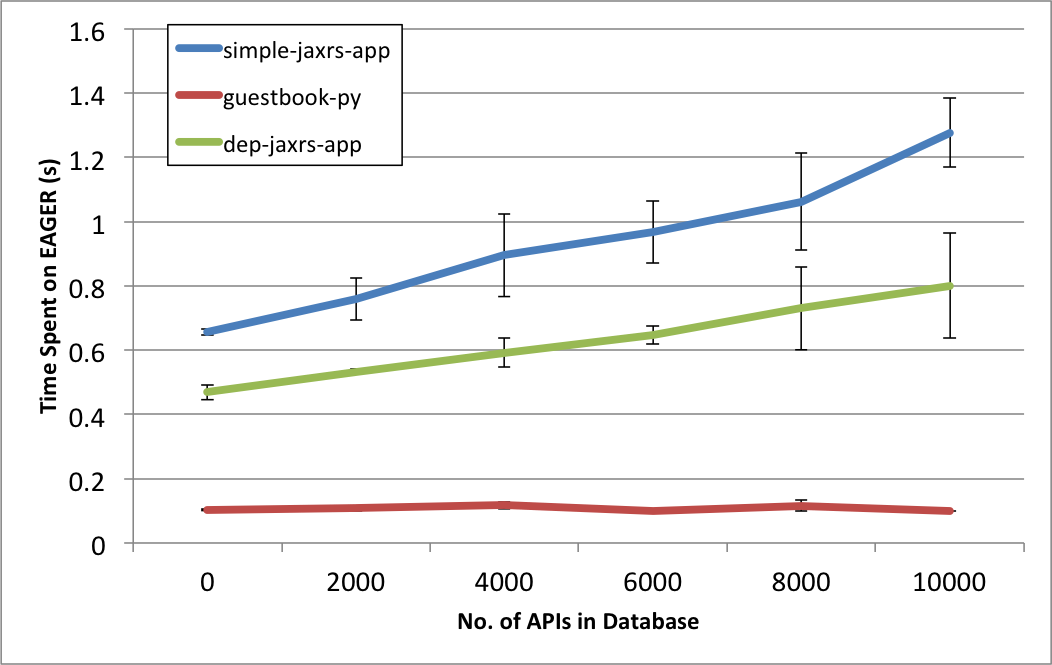
\includegraphics[width=.75\linewidth]{scalability}
  \caption{Overhead vs. number of APIs}
  \label{fig:sub1}
\end{subfigure}%
\begin{subfigure}{.5\textwidth}
  \centering
  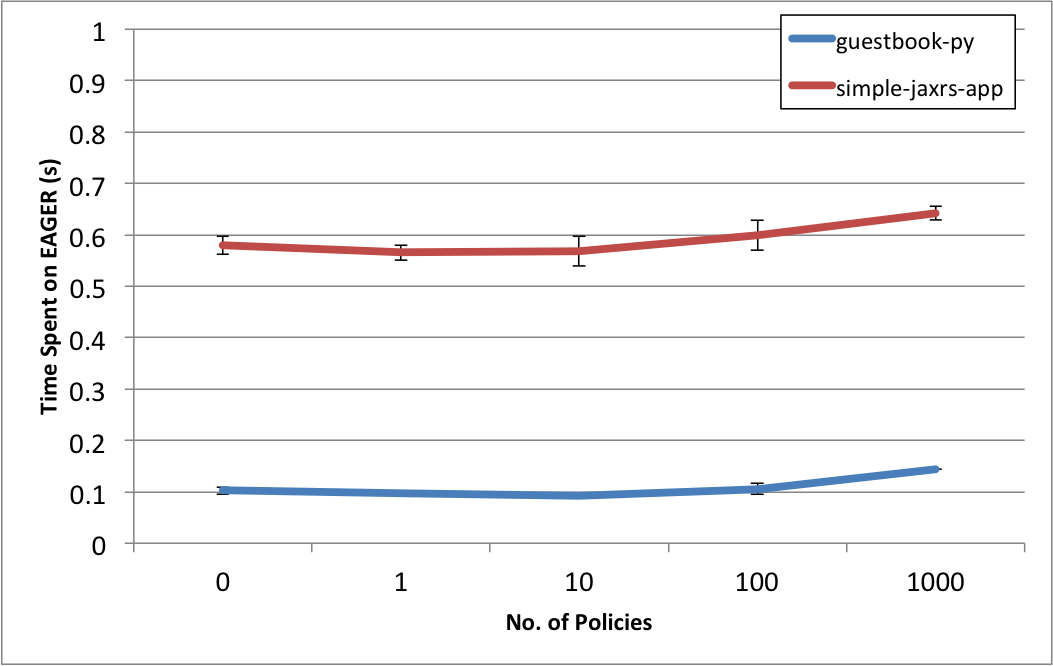
\includegraphics[width=.75\linewidth]{overhead_by_policies}
  \caption{Overhead vs. number of policies}
  \label{fig:sub2}
\end{subfigure}
\caption{EAGER performance overhead and scaling patterns}
\label{fig:eager_perf}
\end{figure}

This research led me to design
EAGER (Enforced API Governance Engine for REST), a 
system that augments PaaS clouds~\cite{6903538}. 
Figure~\ref{fig:eager}  shows EAGER's main components and their interactions.
The Application Deployment Coordinator intercepts all application and API 
deployment requests issued by developers, and validates them against a set of 
admin-specified policies. Applications and APIs are further subjected to a wide 
range of built-in sanity checks, which include an API backwards-compatibility test.
Applications and APIs are only 
hosted in the cloud service runtime, if all the policy and sanity checks return successfully.
Application metadata and historic information required to perform these validations are 
loaded from the Metadata Manager, which gets updated upon each successful deployment
of an application. 
We used a 
restricted subset of Python as the policy specification language, which allows programmers 
to write powerful governance policies in a very simple and intuitive way. EAGER's policy engine 
prevents all I/O operations, most third party library calls, and also global in-memory state, in 
order to perform policy validations in a stateless and side-effect free manner. EAGER also 
supports dependency management and OAuth based authorization for all deployed APIs. 
At run-time EAGER API gateway
intercepts all API calls (requests), and performs authorization and run-time policy validation.

I implemented an initial EAGER 
prototype using the AppScale~\cite{krintzappscale13} open source PaaS (open
source Google App Engine clone).  Like Google App Engine, AppScale
automatically deploys all applications before they execute.  My first
explorations with the EAGER prototype explore its ability to implement
deployment-time governance enforcement on applications that use the Google
App Engine APIs.

To this end, I have modified AppScale so that EAGER is embedded in it.  My
first concern was whether the performance overhead introduced by EAGER would
prohibit its use and adoption.  Using synthetic applications and governance
policies, (i.e. randomized calls and policy predicates) I've profiled EAGER to
determine how invasive its overheads are when its governance checks are
included in the application deployment process.
Figure~\ref{fig:eager_perf}
shows how the EAGER deployment overhead varies for several example web applications, under different
conditions. The time to deploy an application increases slowly as both the
number of APIs EAGER must consider and the number of policies in its governance
database increase.
From these early results, I believe that EAGER will
add negligible overhead to the typical application deployment 
process in the cloud, and can scale to handle thousands of APIs and policies. 
The run-time governance features of EAGER will be further developed and studied in
my future work.

The EAGER deployment-time experiment has prompted me to open a new line of
research exploring the degree to which {\em all} governance policies can be
implemented at deployment-time.  Clearly there are some access control
policies (e.g. those that depend on specific values of parameters passed in an
API call) that must be checked at run-time.  However, I believe it to be an
open question as to what the minimal set of run-time only governance policies
are.

Deployment-time governance implementation
%Currently I'm conducting research in the area of automated performance analysis of web
%services at development time (i.e. before services are deployed into the cloud). This was
%partly inspired by EAGER, which showed that design-time governance
%is not only feasible in clouds, but also 
is desirable for two primary reasons.

\begin{itemize}
%\item APIs are designed and (re)deployed only a few times in their life cycle, whereas they might
%get invoked billions of times once they are in production. Therefore, performing most governance
%checks at design-time of the API avoids repeated work, and scales better in cloud environments.
\item Checking at deployment-time occurs before the application moves into
production execution making its overhead insensitive to the request load 
the application
(or other applications) experience while they are running.  Thus
deployment-time checking does not impede application scaling due to load
(although it may delay application start-up viz. the data shown in
Figure~\ref{fig:eager_perf}).
\item Enforcing most governance policies and sanity checks before the APIs are in production,
prevents the overall cloud system from entering a policy non-compliant state and helps reduce
remediation costs.  In particular, a cloud administrator need not understand
the run-time execution sequence (possibly requiring the assistance of the
application's developer) that causes a policy violation and subsequent failure
of service.
\end{itemize}

\begin{floatingfigure}[rb]{2.8in}
\vspace{-0.1in}
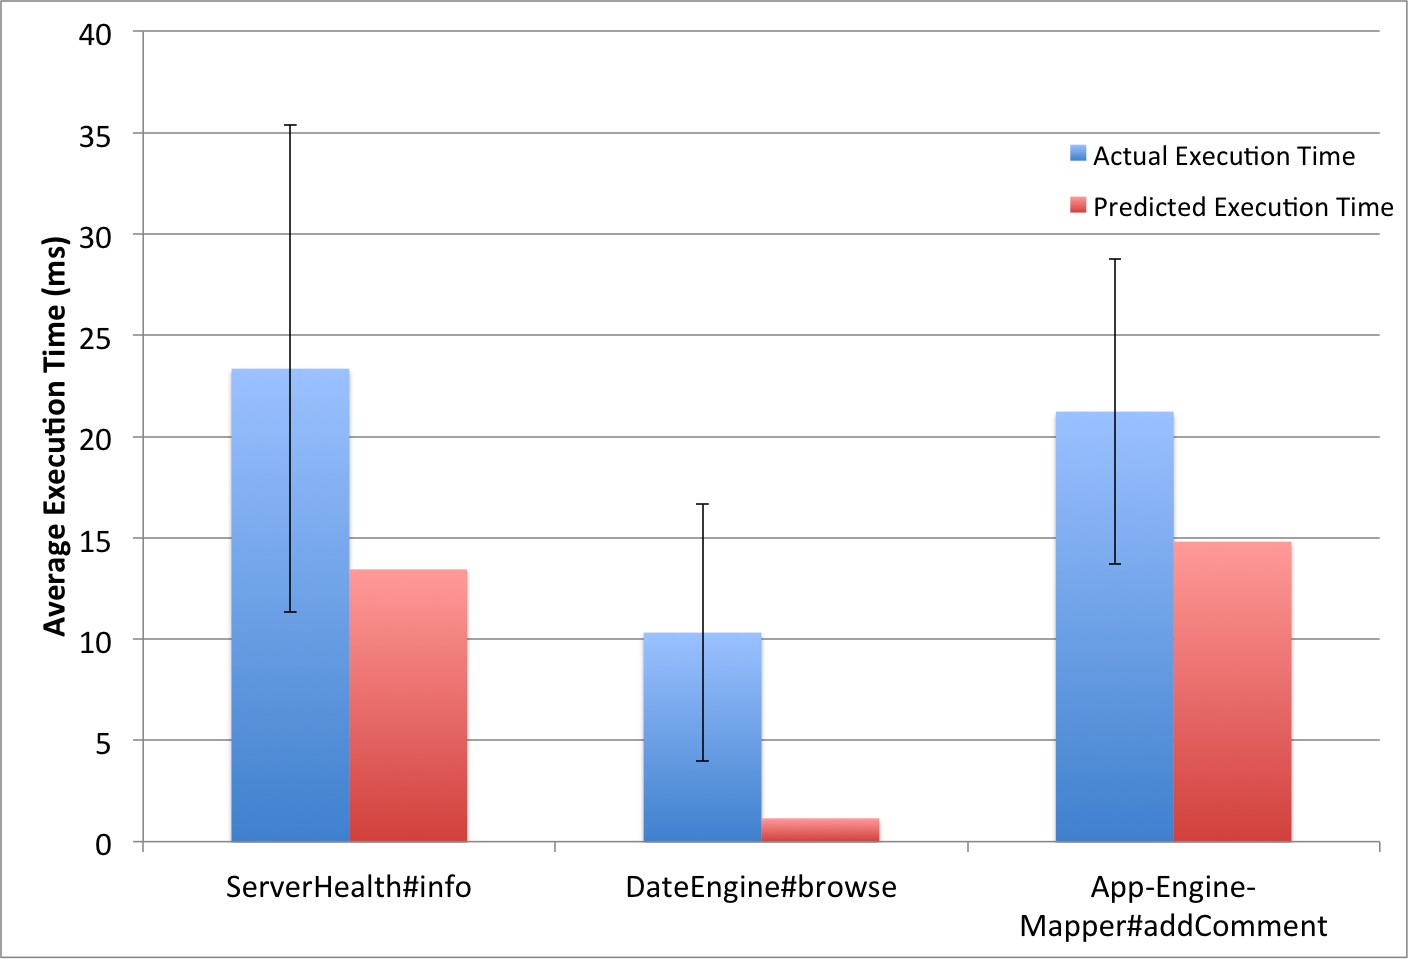
\includegraphics[scale=.27]{static_analysis}
\vspace{-0.08in}
\caption{API performance prediction results\label{fig:static_analysis}}
\end{floatingfigure}

These factors compel me to research what types of policy validations can be 
performed
on web services and APIs before they are deployed in a cloud environment.
In this vein, my current work focuses on deployment-time analysis of 
the application's
ability to meet a run-time SLA once it is deployed.  
I'm attempting to develop methods for analyzing the performance and
QoS traits of APIs at development time, in order to predict their expected performance 
levels early. This is a fairly complex research problem due to the undecidability
inherent in most program analysis tasks. However, cloud environments and SDKs
typically restrict the developers from coding arbitrary services (due to scalability reasons), 
which helps simplify the problem to some extent. Also my early survey results (conducted using
over 100 real world applications developed for PaaS clouds) show that most services developed for
clouds have very few loops and branches, making them highly amenable to static analysis and
verification.

I'm currently using
prominent static analysis methods (abstract interpretation based loop bound analysis,
branch prediction, WCET analysis etc.~\cite{ermedahl_et_al:OASIcs:2007:1194,Yeh:1991:TAT:123465.123475,bygde2010static}) 
to compute paths of execution through service 
implementations. I use this information to build profiles of services which
specify what core cloud services and APIs are being used in a service implementation,
and in which order and frequency. My goal is to combine this information with historical
performance data of the APIs, using simulation methods or other non-parametric statistical
methods~\cite{Nurmi:2007:QQB:1791551.1791556} and derive bounds on the performance expected from the services with high
certainty. 
Such information can be used to formulate SLAs for the services or tune
the service implementations for better performance. 
I have already conducted some preliminary tests in this area using real world
Java web applications developed for the Google App Engine (and AppScale) environment,
and the initial results are quite encouraging. Figure~\ref{fig:static_analysis} shows the actual
execution time of three services and the predicted executions times of the same obtained using
a bare bones implementation of my static analysis-based approach (which is still in its infancy). 
It is interesting
to see that even without any optimizations, the predictions generated by my approach are 
within the acceptable deviation range of the actual values in two out of the three services considered.
Predictions made on the DateEngine application are somewhat off from the acceptable range, due
to its excessive use of JSP and other user interface code, which are currently not analyzed by
my static analyzer.
In the future I intend to further extend 
these methods to perform SLA management and enforcement both at design-time and run-time.


\section{Conclusion}
Cloud computing delivers IT infrastructure resources, programming platforms, and software
applications as shared utility services. Enterprises and developers increasingly deploy applications 
on cloud platforms due to their scalability, high availability and many other
productivity enhancing features. Cloud-hosted applications depend on the core services provided
by the cloud platform for compute, storage and network resources. 
In some cases they use the services provided by the cloud to implement most of
the application functionality as well (e.g. PaaS-hosted applications). 
Cloud-hosted applications are typically
accessed over the Internet, via the web APIs exposed by the applications.

As the applications hosted in cloud platforms continue to increase in number, the need for enforcing
governance on them becomes accentuated. We define governance as the mechanism by which the 
acceptable operational parameters are specified and maintained for a cloud-hosted application.
Governance enables specifying the acceptable
development standards and runtime parameters (performance, availability, security requirements etc.) 
for cloud-hosted applications as policies. Such
policies can then be enforced automatically at various stages of the application life-cycle. 
Governance also entails
monitoring cloud-hosted applications to ensure that they operate at a certain level of quality,
and taking corrective action when deviations are detected. Through the steps of specification,
enforcement, monitoring and correction, governance facilitates resolving a number of prevalent issues in
today's cloud platforms. These issues include lack of good software engineering practices (code reuse,
dependency management, versioning etc), lack of performance SLOs for cloud-hosted applications,
and lack of performance debugging support. 

We explore the feasibility of efficiently enforcing governance on cloud-hosted
applications, and evaluate the effectiveness of governance as a means of achieving administrative
conformance, developer best practices and performance SLOs in the cloud. Considering the scale of
today's cloud platforms in terms of the number of users and the applications, 
we strive to automate much of the governance tasks through
automated analysis and diagnostics. To achieve efficiency, we put more emphasis on deployment-time
policy enforcement, static analysis of performance bounds, and non-invasive passive monitoring of 
cloud platforms, thereby keeping the governance overhead
to a minimum. We avoid run-time enforcement and invasive instrumentation of cloud applications 
as much as possible. We also focus on building governance systems that are deeply integrated with
the cloud platforms themselves. This enables using the existing scalability and high availability features of the cloud
to provide an efficient governance solution that can control all application events in a fine-grained
manner. Furthermore, such integrated solutions relieve the users from having to maintain and pay
for additional, external governance and monitoring solutions.

In order to explore the feasibility of implementing efficient, automated governance systems in 
cloud environments, and evaluate the efficacy of such systems, we follow a three-step
research plan.
\begin{enumerate}
\item Design and implement a scalable, low-overhead policy enforcement system for cloud platforms.
\item Design and implement a methodology for formulating performance SLOs for cloud-hosted applications.
 \item Design and implement a scalable application performance monitoring system for 
 detecting and diagnosing performance anomalies in cloud platforms.
\end{enumerate}

We design and implement EAGER~\cite{6903538, eager-fop15} -- a lightweight governance policy
enforcement framework built into PaaS clouds. It supports defining policies using a simple syntax
based on the popular Python programming language. EAGER promotes deployment-time
policy enforcement, where policies are enforced on user applications (and APIs) every time
an application is uploaded to the cloud. By carrying out policy validations at
application deployment-time, and refusing to deploy applications that violate policies,
 we provide fail-fast semantics, which ensure that deployed applications are fully policy compliant. 
EAGER architecture also provides the necessary provisions for facilitating run-time policy
enforcement (through an API gateway proxy) when necessary. This is required, since not all
policy requirements are enforceable at deployment-time; e.g. a policy that prevents an
application from making connections to a specific network address. Our experimental results show
that EAGER validation and policy enforcement overhead is negligibly small, and it scales well to
handle thousands of user applications and policies. Overall, we show that integrated governance
for cloud-hosted applications is not only feasible, but also can be implemented with very
little overhead and effort.

To facilitate formulating performance SLOs, we design and implement 
Cerebro~\cite{Jayathilaka:2015:RTS:2806777.2806842} --
a system that predicts bounds on the response time of web applications developed for PaaS clouds.
Cerebro is able to analyze a given web application, and determine a bound on its response time without
subjecting the application to any testing or runtime instrumentation. This is achieved by a mechanism
that combines static analysis of application source code with runtime monitoring of the underlying
cloud platform (PaaS SDK to be specific). Our approach is limited to interactive web applications
developed using a PaaS SDK. We show that such applications have very few branches and loops, 
and they spend most of their execution time invoking PaaS SDK operations. These properties
make the applications amenable to both static analysis, and statistical treatment of their 
performance limits.

Cerebro is fast, can be invoked at the deployment-time 
of an application, and does not require any human input or intervention. 
The bounds predicted by Cerebro can be used as statistical guarantees (with well defined correctness
probabilities) to form performance SLOs. These SLOs in turns can be used in SLAs that are negotiated
with the users of the web applications. Cerebro's SLO prediction capability, coupled with a policy
enforcement framework such as EAGER, can facilitate specification and enforcement of performance-related
policies for cloud-hosted applications. We implement Cerebro for Google App Engine public cloud
and AppScale private cloud. Our experiments with real world PaaS applications show that Cerebro
is able to determine accurate performance SLOs that closely reflect the actual response time
of the applications. Furthermore, we show that Cerebro-predicted SLOs are not easily affected by
the dynamic nature of the cloud platform, and they remain valid for long durations. More specifically, 
Cerebro predictions remain correct for more than 12 days on average~\cite{7396174}. 

Finally, we design and implement Roots -- a performance anomaly detection and 
bottleneck identification system built into PaaS clouds. It collects data from all the different layers of the
PaaS stack; from load balancers to low level PaaS kernel service implementations. However,
it does so without instrumenting user code, and without introducing a significant
overhead to the application request processing flow. 
Roots uses the metadata (request identifiers) injected by the load balancers to correlate the
events observed in different layers, 
thereby enabling tracing of application requests through the PaaS stack.
Roots is also extensible in the sense that 
any number of statistical analysis methods can be incorporated into Roots for performance
anomaly detection and diagnosis. Furthermore, it facilitates configuring monitoring requirements
at the granularity of user applications, which allows different applications to be monitored
and analyzed differently. 

Roots detects performance anomalies by monitoring applications for performance SLO violations. 
When an anomaly (i.e. an SLO violation) is detected, Roots determines if
the anomaly was caused by a change in the application workload or by a performance 
bottleneck in one of the underlying PaaS kernel services. If the SLO violation was caused by
a performance bottleneck in the cloud, Roots needs to be able to locate the exact PaaS kernel
service in which the bottleneck manifested. To this end we present a root cause analysis method
that uses a combination of linear regression, change point detection and quantile analysis.
We show that our combined methodology makes accurate diagnoses nearly
100\% of the time. Moreover, we also present a path distribution analyzer that can identify different
paths of execution in an application, via the run-time data gathered from the cloud platform.
We show that this mechanism is capable of detecting characteristic changes in application
workload as a special type of anomalies.

Our results demonstrate that efficient and automated governance in cloud environments
is not only feasible, but also highly effective. We did not have to implement a cloud platform from the 
scratch to implement the governance systems designed as a part of this work. Rather,
we were able to implement the proposed governance systems for existing cloud platforms
like Google App Engine and AppScale; often with minimal changes to the cloud platform
software. Our policy enforcement and monitoring systems are integrated with the cloud platform 
(i.e. they operate from within the cloud platform), and hence preclude 
the cloud platform users from having to set up or
implement their own external governance solutions that provide API management or
application monitoring functionality. Our governance systems are also efficient, in the 
sense they do not add a significant overhead to the applications deployed in the cloud
platform, and they scale well to handle a very large number of applications and governance
policies.

Our research is aimed at providing increased levels of oversight, control and automation
to cloud platforms. Therefore it has the potential
to increase the value offered by the cloud platforms to the application developers
and the application clients. More specifically, our research can greatly enhance the
use of PaaS clouds. A lot of our work is directly applicable to popular PaaS clouds
such as Google App Engine and AppScale, and the respective developer communities
can greatly benefit from our findings.

Our research paves the way to making cloud platforms more dependable and 
maintainable for administrators, application developers and clients alike. It brings
automated policy enforcement -- a governance technique that has been successfully applied
in classic SOA systems in the past -- to modern cloud environments. Policy enforcement
solves a variety of issues related to poor application coding practices, and lack
of administrative control. We also enable stipulating performance SLOs for
cloud-hosted applications, a feature that is not supported in existing cloud platforms
to the best of our knowledge. Our research also supports full-stack monitoring of cloud
platforms for detecting performance SLO violations, and determining the root causes
of such violations. When taken together, our research addresses all three
components of governance (specification, enforcement and monitoring) both 
efficiently and automatically, as cloud-native features. The systems we propose
ensure that cloud-hosted applications always operate in a policy compliant state,
and any performance anomalies are detected and diagnosed fast.
In conclusion, our governance systems facilitate achieving developer best practices, 
administrative conformance and performance SLOs for cloud-hosted applications in ways
that were not possible before.

\end{document}
